\documentclass[12pt, a4paper]{article}  

\usepackage{etex} % расширение классического tex в частности позволяет подгружать гораздо больше пакетов, чем мы и займёмся далее

%%%%%%%%%% Математика %%%%%%%%%%
\usepackage{amsmath,amsfonts,amssymb,amsthm,mathtools} 
%\mathtoolsset{showonlyrefs=true}  % Показывать номера только у тех формул, на которые есть \eqref{} в тексте.
%\usepackage{leqno} % Нумерация формул слева


%%%%%%%%%%%%%%%%%%%%%%%% Шрифты %%%%%%%%%%%%%%%%%%%%%%%%%%%%%%%%%
\usepackage{fontspec}         % пакет для подгрузки шрифтов
\setmainfont{Arial}   % задаёт основной шрифт документа

\defaultfontfeatures{Mapping=tex-text}

% why do we need \newfontfamily:
% http://tex.stackexchange.com/questions/91507/
\newfontfamily{\cyrillicfonttt}{Arial}
\newfontfamily{\cyrillicfont}{Arial}
\newfontfamily{\cyrillicfontsf}{Arial}

\usepackage{unicode-math}     % пакет для установки математического шрифта
\setmathfont{Asana Math}      % шрифт для математики

\usepackage{polyglossia}      % Пакет, который позволяет подгружать русские буквы
\setdefaultlanguage{russian}  % Основной язык документа
\setotherlanguage{english}    % Второстепенный язык документа
\usepackage{icomma} % "Умная" запятая: $0,2$ --- число, $0, 2$ --- перечисление

%% Номера формул
%\mathtoolsset{showonlyrefs=true} % Показывать номера только у тех формул, на которые есть \eqref{} в тексте.

%% Шрифты
\usepackage{euscript}	 % Шрифт Евклид
\usepackage{mathrsfs} % Красивый матшрифт
\usepackage{enumitem,xcolor}
\usepackage{indentfirst}  
\usepackage{float}
\usepackage{chngcntr} %обнуляет счетчики рисунков для новой главы
\counterwithin{figure}{section}
\usepackage{etoolbox}
\usepackage{scrextend}

%% Свои команды
\def \a{\alpha}
\def \R{\ensuremath{\mathbb{R}}}
\DeclareMathOperator{\sgn}{\mathop{sgn}}
\newcommand{\bb}[1]{\ensuremath{\mathbb{#1}}}%определение новых команд
\renewcommand{\phi}{\varphi}%переопределние существующих команд
\DeclareMathOperator{\Var}{Var}
\DeclareMathOperator{\Cov}{Cov}
\newcommand{\s}{\ensuremath{\sigma}}
\newcommand{\mdot}{\ensuremath{x_1 \ldots x_n}}
\newcommand{\com}[2]{\ensuremath{x_{#1} \ldots x_{#2}}}
\newcommand{\llim}[2]{\ensuremath{\lim\limits_{#1} #2}}
\renewcommand{\thefigure}{\arabic{section}:\arabic{figure}}
\renewcommand{\theequation}{Eq.(\arabic{equation})}


%% Перенос знаков в формулах (по Львовскому)
\newcommand*{\hm}[1]{#1\nobreak\discretionary{}
{\hbox{$\mathsurround=0pt #1$}}{}}


%%% Заголовок
\title{Tikz in \LaTeX}
\date{\today}

\begin{document} % конец преамбулы, начало документа
\renewcommand{\thepage}{\ifthispageodd{\Asbuk{page}}{\Roman{page}}} %уродская нумерация

\maketitle
\noindent \ignorespaces

\section{Команды}

$\Var(\bar{x})=\frac{\sigma^2}{n}$ \\
$\Cov (x_t ; x_{t+k}) = \gamma_k$ \\
\s--алгебра\\

\mdot \quad
\com{1}{6} \quad \com{a}{z} \quad \com{(a,b)}{(c,d)} \\

\begin{itemize}[label=\textcolor{blue}{\textbullet}]
\item Первый пункт
\item Второй пункт
\item Третий пункт
\end{itemize}

\llim{x\to 0}{\frac{\sin x}{x}} 

\newpage

\section{Cчетчики}

\begin{figure}[H] 
\centering
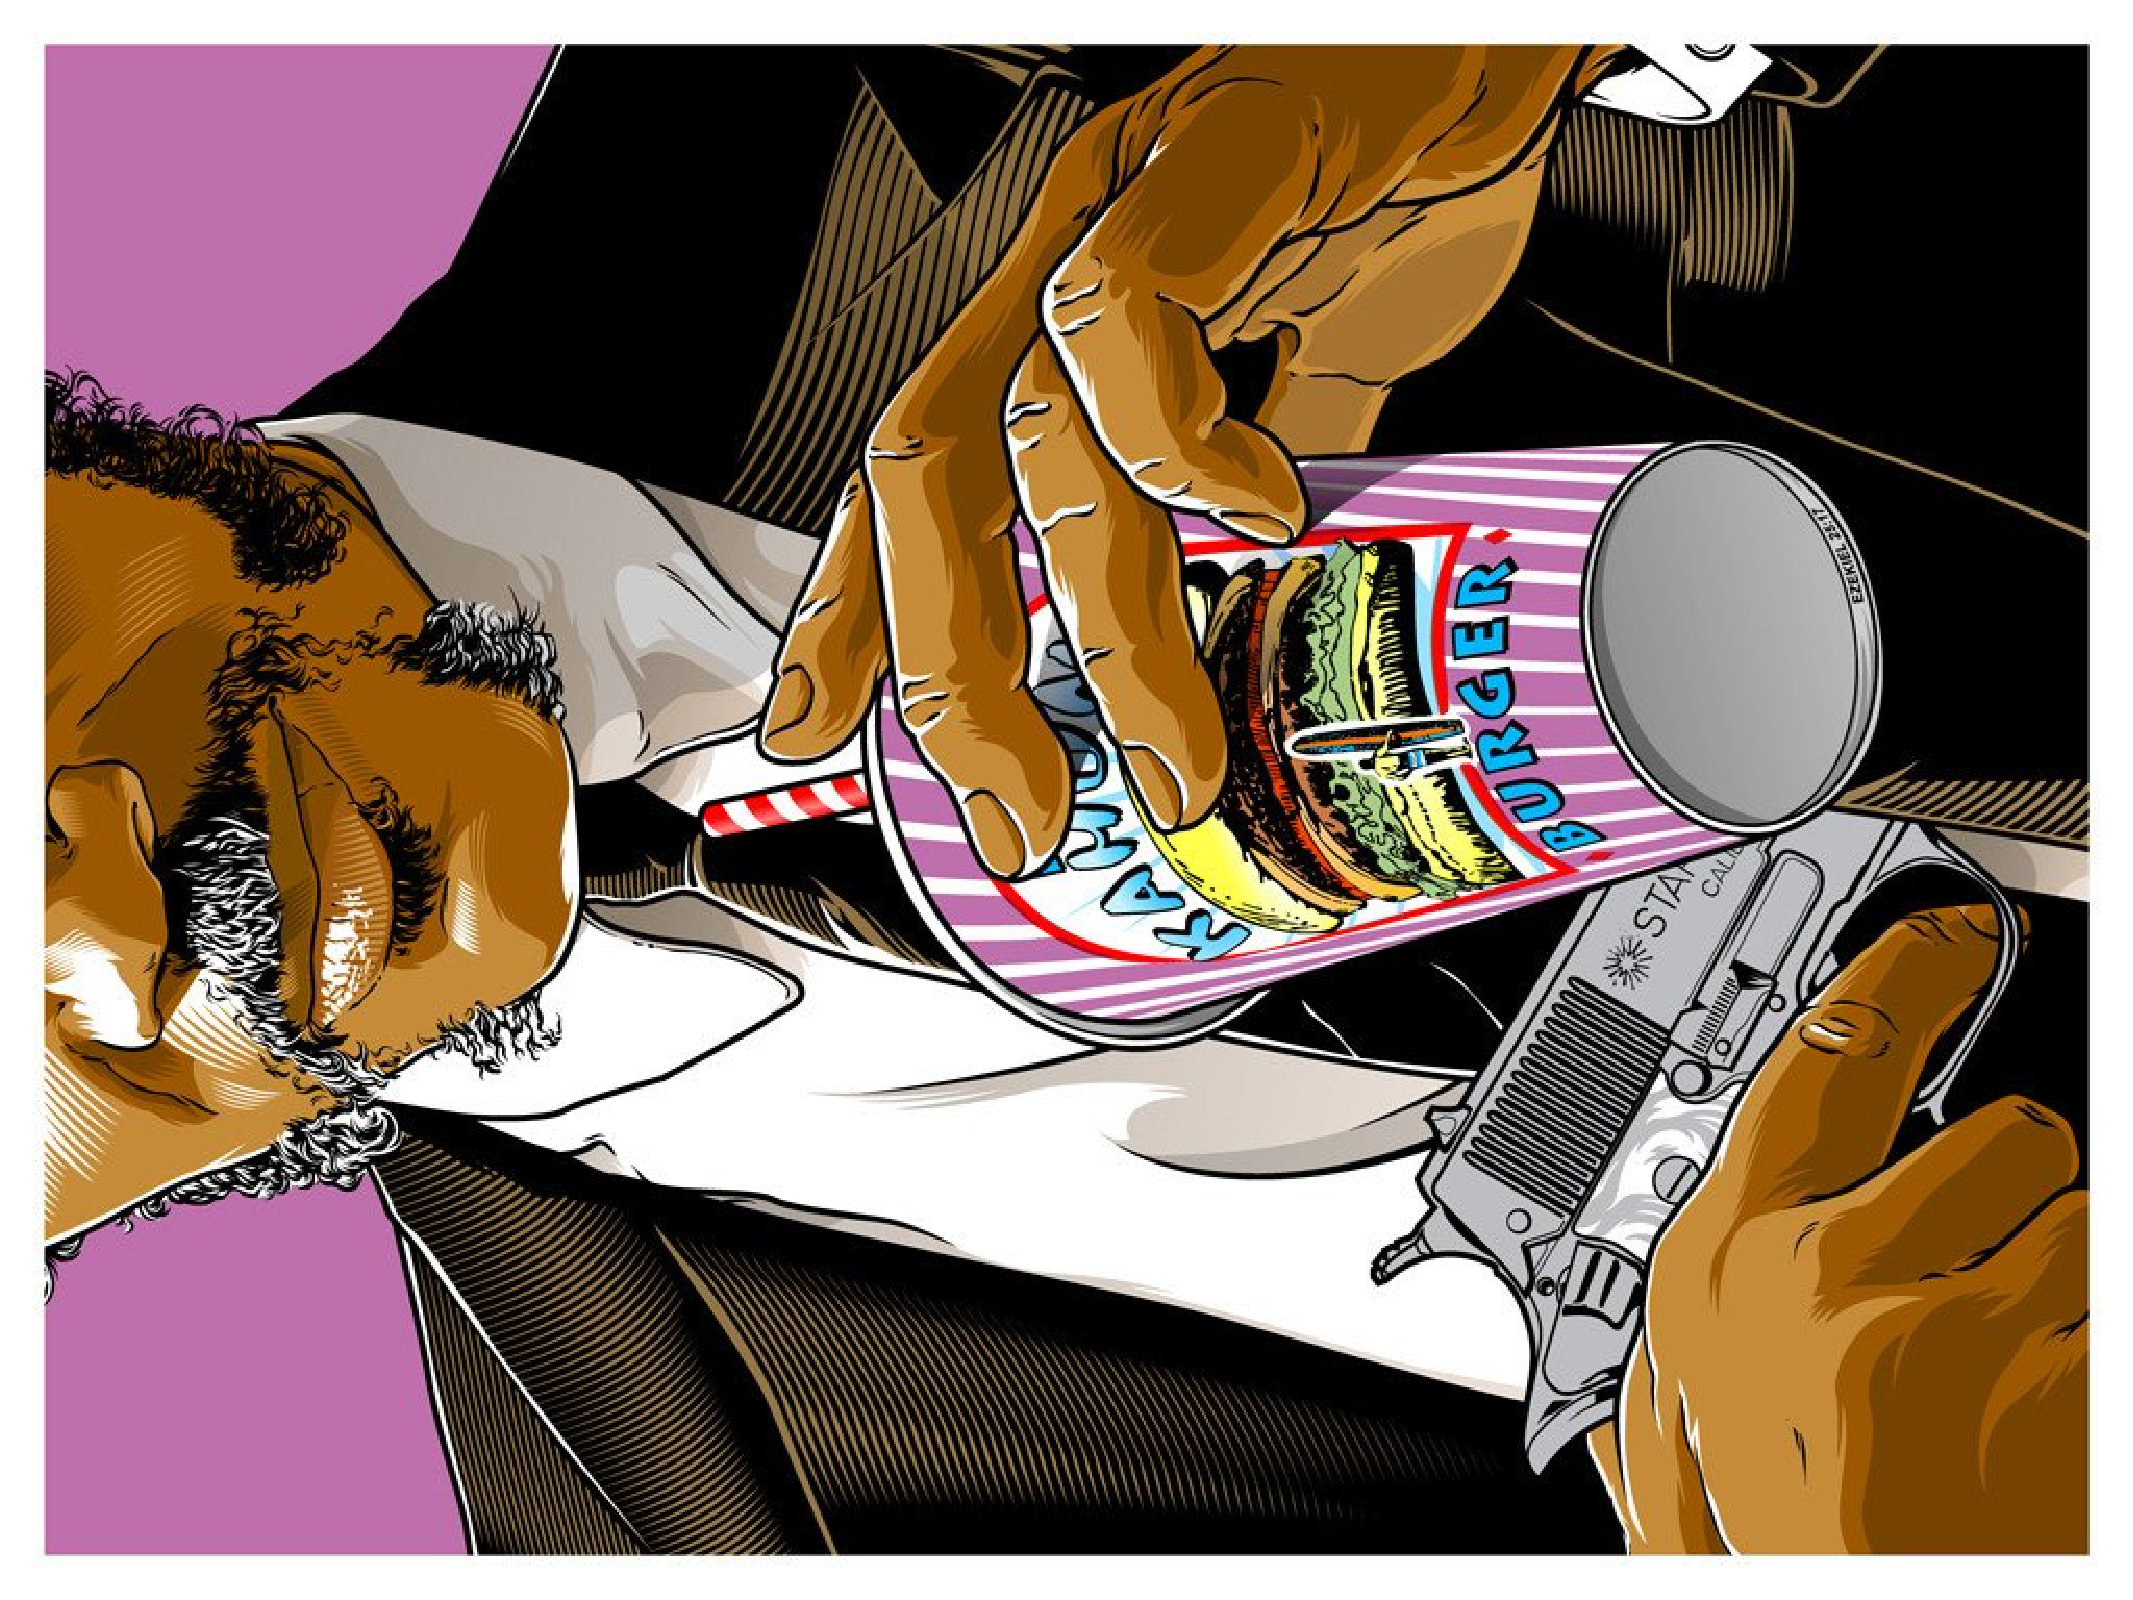
\includegraphics[width=0.3\paperwidth, angle=270]{pop1.pdf}
\caption{Pulp fiction}  \label{fig:3}
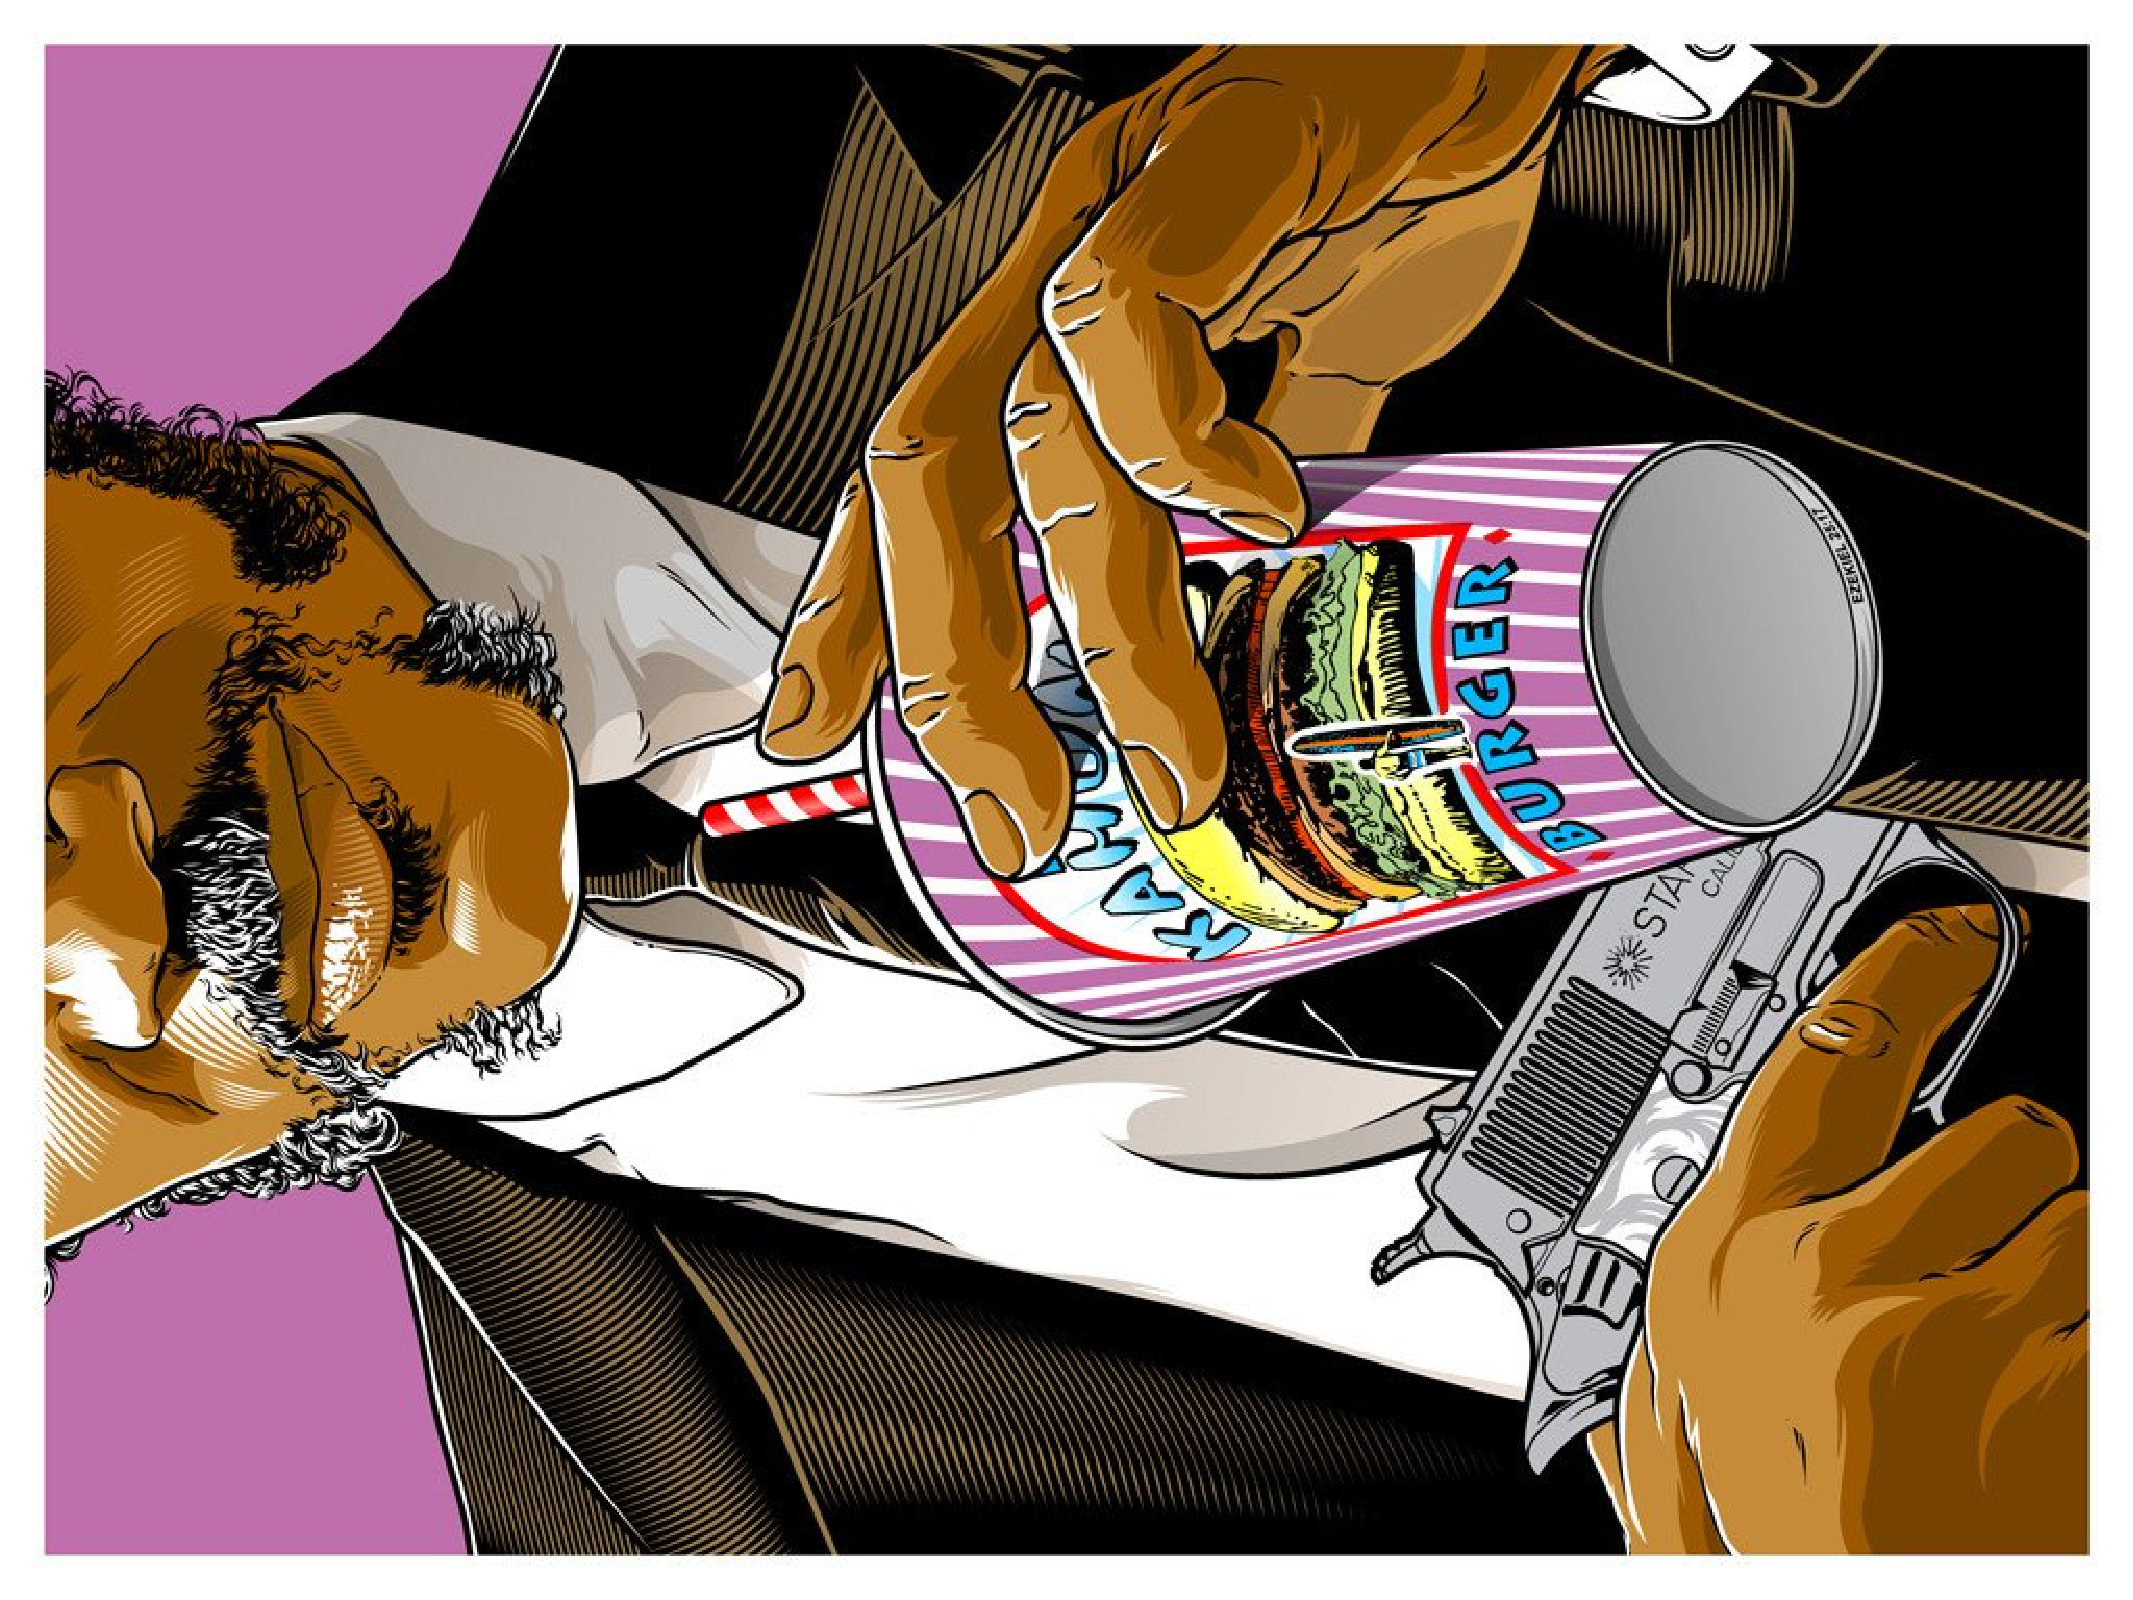
\includegraphics[width=0.3\paperwidth, angle=270]{pop1.pdf}
\caption{Pulp fiction} \label{fig:1}
\end{figure} 

На рисунке \ref{fig:3} то же самое, что и на рисунке \ref{fig:1} \\

\begin{equation}
\Cov (x_t ; x_{t+k}) = \gamma_k
\end{equation}

\newpage

\section{Дургие команды}
\newcommand{\crazy}[1]{\scalebox{-1}[-1]{#1}}
\crazy{Хочу шаурму} \\ %перевертыш

\newcommand{\AR}[1]{\ensuremath {X_t=\varepsilon_t + \sum_{k=0}^{#1}a_k X_{t-k}}}  %Авторегрессия
\AR{3} \\

\newcommand{\MA}[1]{\ensuremath {X_t=\varepsilon_t + \sum_{k=1}^{#1}b_k \varepsilon_{t-k}}} %скользящее средние
\MA{5} \\

\newcommand{\ARMA}[2]{\ensuremath {X_t=\sum_{k=1}^{#1}a_k X_{t-k} + \sum_{k=0}^{#2}b_k \varepsilon_{t-k}}} 
\ARMA{2}{3}



\end{document}
